\documentclass[11pt]{beamer}

\usepackage{url}
\usepackage{tikz}
\author{Armijn Hemel\\Tjaldur Software Governance Solutions}
\title{What goes into a binary?}
\date{October 28, 2011}

\begin{document}

\setlength{\parskip}{4pt}

\frame{\titlepage}

\frame{
\frametitle{About Armijn}

\begin{itemize}
\item using Open Source software since 1994
\item MSc Computer Science from Utrecht University (The Netherlands)
\item core team \url{gpl-violations.org} since 2005
\item ex-board member at NLUUG (\url{http://www.nluug.nl/})
\item sysadmin, developer and consultant at Loohuis Consulting (2006 - May 2011)
\item May 2011 - present: owner Tjaldur Software Governance Solutions
\end{itemize}
}

\frame{
\frametitle{Our research \& this talk}
We argue:

\begin{itemize}
\item not granular enough: for example package information in distributions is too coarse and often incorrect
\item static (source code) analysis alone is not enough to determine the right license of a binary
\item we all need to do a better job
\end{itemize}

This is not (necessarily) a pure licensing talk! One of the applications is related to licensing, so focus will be on that.

Also: this is unpublished research (sent to International Conference on Software Engineering 2012), so still rough.
}

\frame{
\frametitle{The team}

\begin{itemize}
\item Eelco Dolstra (Delft University of Technology, the Netherlands)
\item Sander van der Burg (Delft University of Technology, the Netherlands)
\item Daniel M. German (University of Victoria, Canada)
\item Julius Davies (University of Victoria, Canada)
\item Armijn Hemel (Tjaldur Software Governance Solutions, the Netherlands)
\end{itemize}

WANAL
}

\frame{
\frametitle{Licensing is hard}
Doing correct licensing is not trivial and there are many unclarities:

\begin{itemize}
\item Linux kernel
\item Amarok
\item KDE
\item \texttt{opkg}
\end{itemize}
}

\frame{
\frametitle{Example: Linux kernel}
GPLv2 licensed, or is it?

\begin{quote}
This program is free software; you can redistribute it and/or modify
it under the terms of the GNU General Public License as published by
the Free Software Foundation, version 1
\end{quote}

(source: \texttt{drivers/net/cs89x0.h})
}

\frame{
\frametitle{Example: Amarok}
Amarok is a popular music player originating from KDE, licensed as GPLv2+ (with KDE exceptions).

For two years some files were GPLv3+ by accident because of a typo.
}

\frame{
\frametitle{Example: KDE}
What license is this?

\begin{quote}
This library is free software; you can redistribute it and/or
modify it under the terms of the GNU Library General Public
License as published by the Free Software Foundation version 2.0
\end{quote}

(source: \texttt{kioslave/metainfo/metainfo.cpp} in \texttt{kdelibs})

It is very likely they actually meant LGPL 2.

In short: many projects have suboptimal, or unclear (or no) license statements. We can do better here!
}

\frame{
\frametitle{Example: \texttt{opkg}}
\texttt{opkg} is a package manager that is used on embedded Linux distributions.

Question: given a binary of \texttt{opkg}, what license(s) can it be distributed
under?
}

\frame{
\frametitle{GPLv2? GPLv2+? GPLv3+?}
\texttt{opkg} has a \texttt{COPYING} file containing the text of GPLv2.

All source code files in \texttt{opkg} are GPLv2+ \textbf{except} \texttt{libopkg/sha256.c} and \texttt{libopkg/sha256.h} which are GPLv3+!

These files are not always included, but they are most of the time. The \texttt{configure} script has a switch:

\texttt{\\   --enable-sha256         Enable sha256sum check [default=yes]\\}


Correct answer: it depends and more information about the \texttt{composition} of the binary is needed.
}

\frame{
\frametitle{Possible solution: static analysis?}
Static analysis (source code level) can tell you a lot, but information is vastly incomplete:

\begin{itemize}
\item many different types of build systems and scripts
\item output from \texttt{configure} has huge influence
\item environment variables set by scripts or users
\end{itemize}
}

\frame{
\frametitle{Better solution: tracing the build}
We can track system calls using \texttt{strace} and see which files are used by a build!

\begin{itemize}
\item no need to modify existing build tools
\item (pretty much) standard package for Linux
\item build system agnostic
\item no special privileges needed
\end{itemize}

Minor drawbacks:

\begin{itemize}
\item a bit verbose
\item performance hit
\end{itemize}
}

\begin{frame}[fragile]
\frametitle{Trace example output}
\begin{verbatim}
  open("patchelf.cc", O_RDONLY)
  open("/usr/include/c++/4.5.1/string",
    O_RDONLY|O_NOCTTY)
  open("elf.h", O_RDONLY)
\end{verbatim}
\end{frame}

\begin{frame}[fragile]
\frametitle{Result: build graph}

\includegraphics[width=1.0\columnwidth]{example}
\end{frame}

\frame{
\frametitle{Pruning the result graph}
Only tracing which files are used gives a \textit{conservative} estimate of which files are used.

False positives (files that are opened, but not used for building the actual binary) can be pruned by adding more intelligence.
}

%\frame{
%\frametitle{Applications}
%Use result set:
%
%\begin{itemize}
%\item determine license of each file (using Ninka, or FOSSology)
%\item scan for security bugs
%\item \dots
%\end{itemize}
%}

\frame{
\frametitle{Early success: \texttt{FFmpeg}}
\texttt{FFmpeg} is a mix of GPLv2+ and LGPLv2.1+ licensed code. The \texttt{configure} script has an option to only use the LGPLv2.1+ sources for a build.

With our approach we found that some GPLv2+ code was \textit{always} included in \texttt{libavfilter}.

The offending code was in \texttt{libavfilter/x86/gradfun.c}, licensed under the GPLv2+.

This was not trivial to find out from the \texttt{FFmpeg} build scripts.

\texttt{FFmpeg} fixed it within hours after being informed.
}

\begin{frame}[fragile]
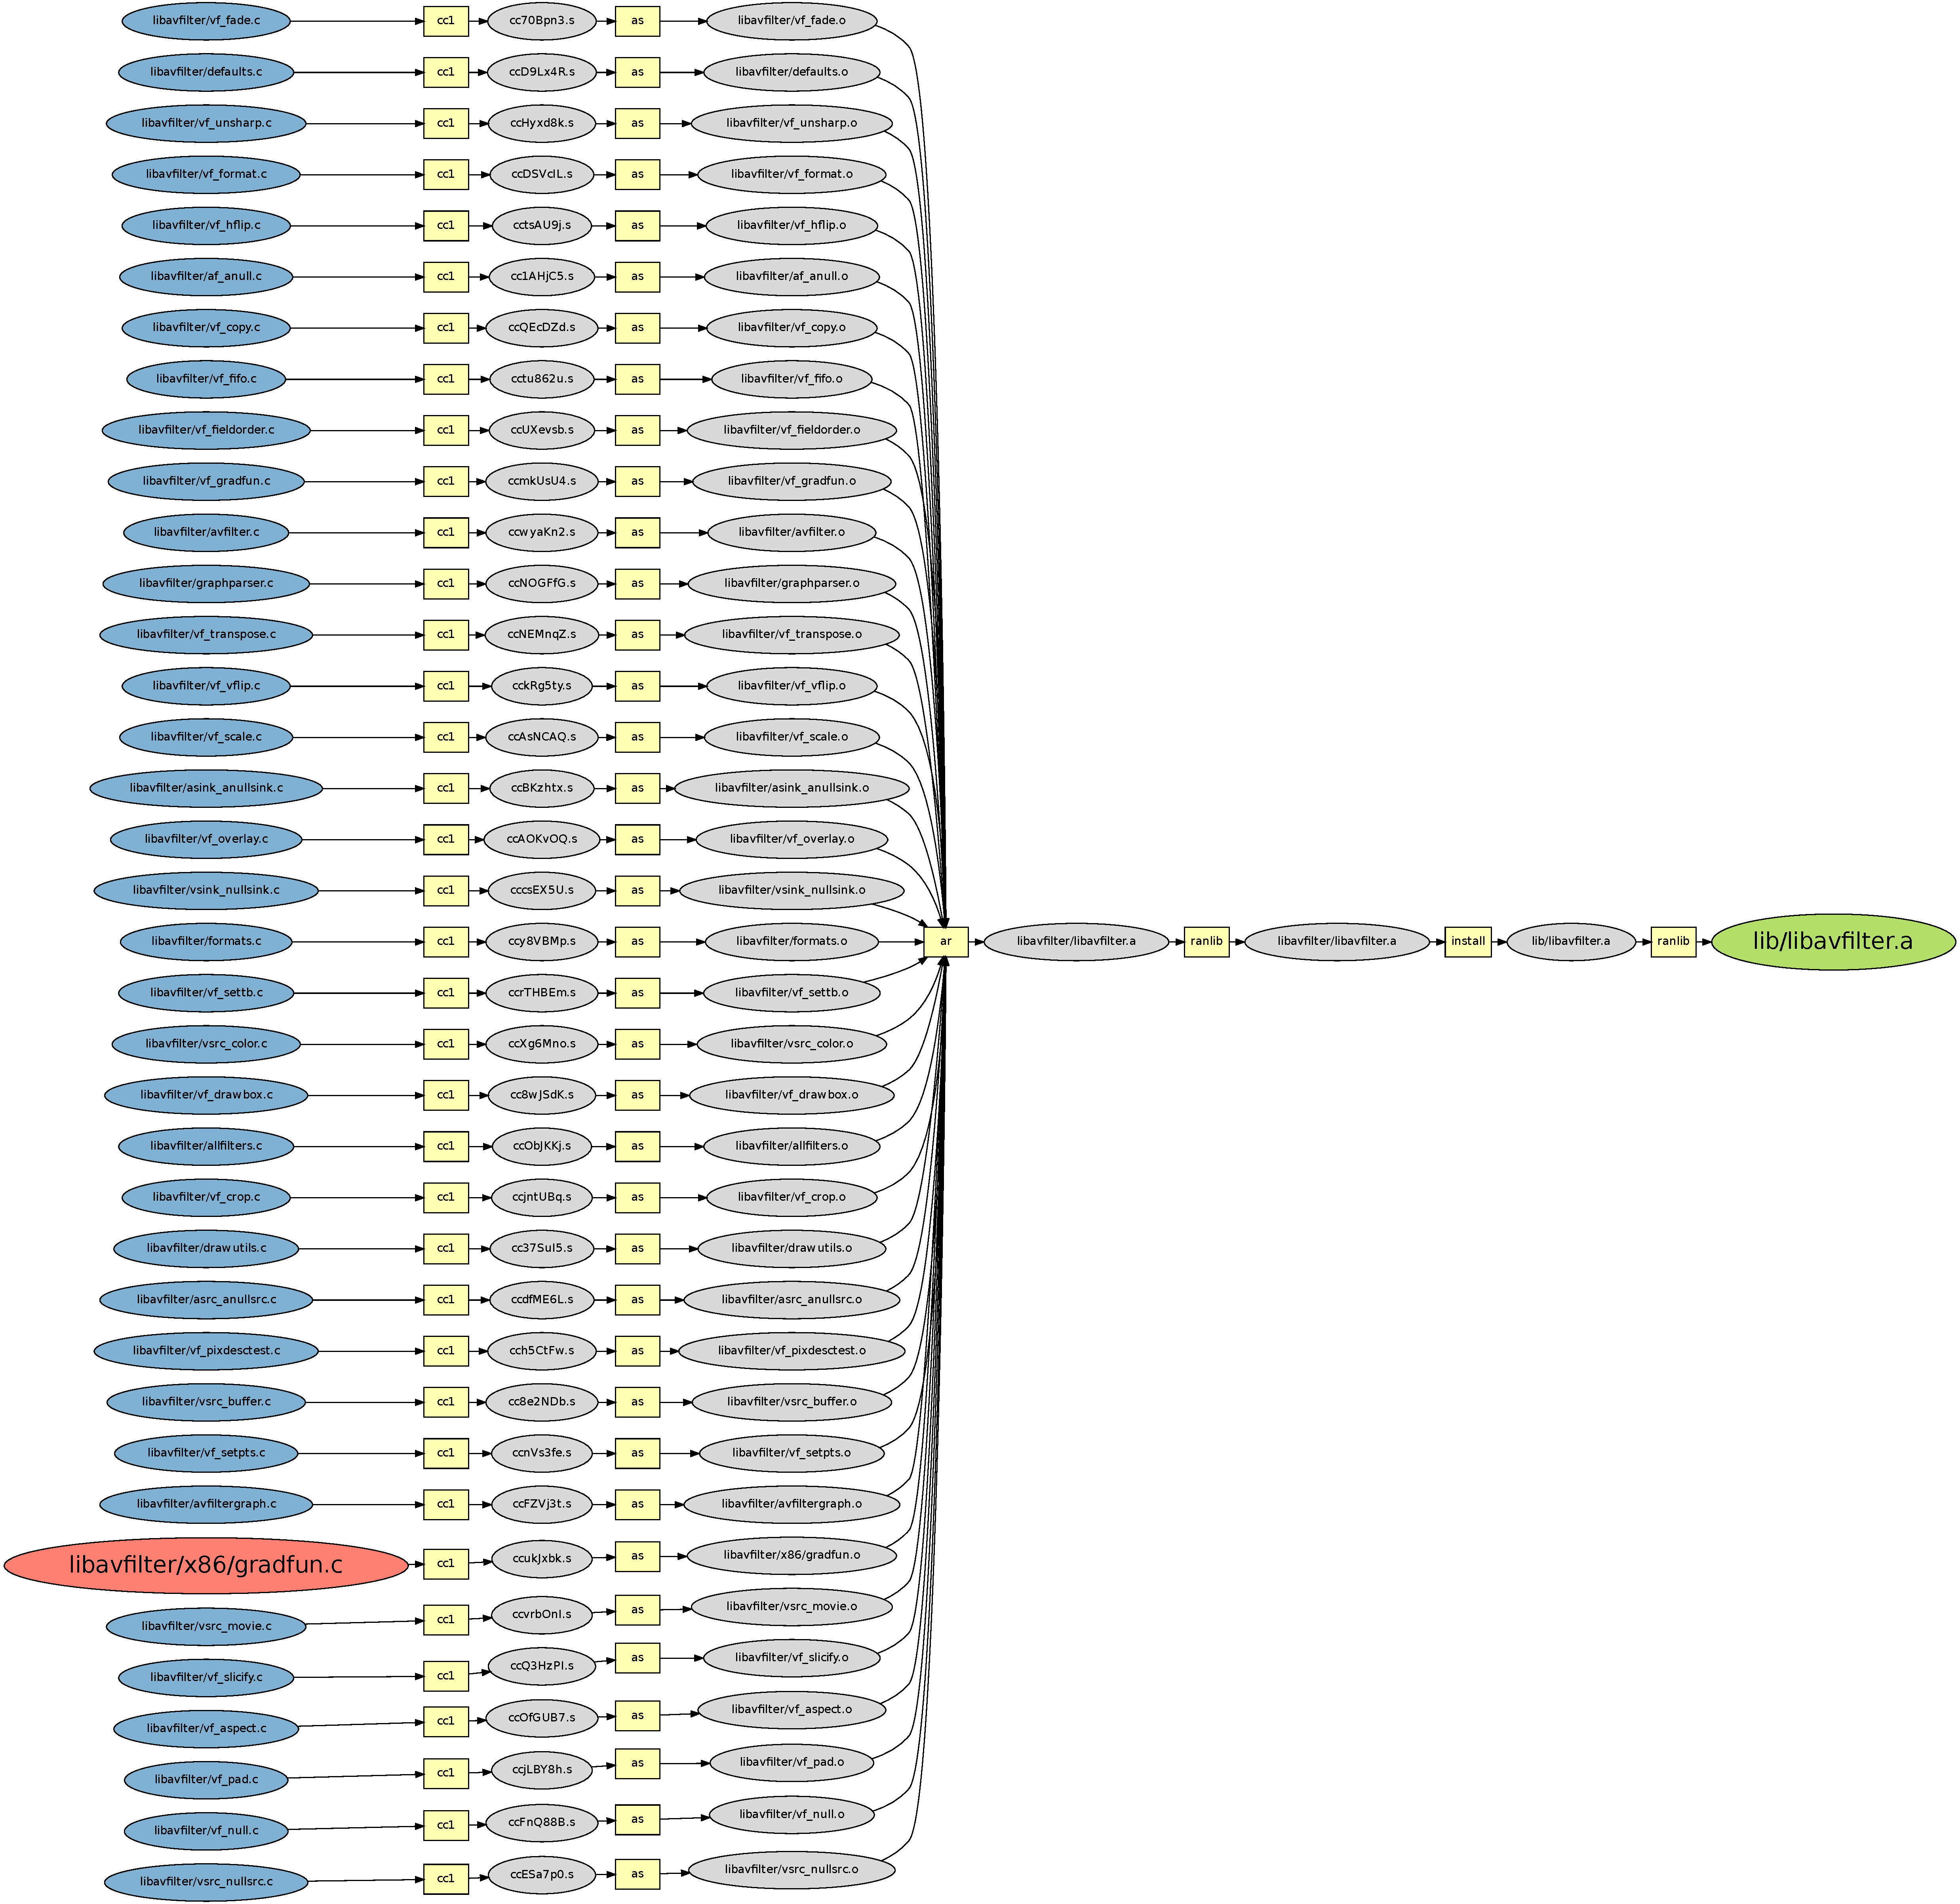
\includegraphics[width=0.9\columnwidth]{ffmpeg_no_gpl_libavfilter_crop}
\end{frame}

\frame{
\frametitle{Is this enough?}
Nope, because we only consider \textit{build time} composition.

Two important things to consider:

\begin{itemize}
\item run time composition
\item license granularity
\end{itemize}
}

\frame{
\frametitle{Run time composition}

\begin{itemize}
\item dynamic linking (run time)
\item dynamically loading files
\item RPC/networked services
\end{itemize}
}

\frame{
\frametitle{License granularity}
Licenses can also apply to parts of files:

\begin{quote}
 * Kuhn's copyrights are licensed GPLv2-or-later.  File as a whole remains GPLv2.
\end{quote}

(source: \texttt{wget.c} in recent BusyBox)

\begin{quote}
 * The md5\_crypt() function was taken from freeBSD's libcrypt and contains \\
 * this license: \\
 *    "THE BEER-WARE LICENSE" (Revision 42):
\end{quote}

(source: \texttt{libcrypt/md5.c} in uClibc)
}

\frame{
\frametitle{Conclusions}

\begin{itemize}
\item licensing in Open Source software projects is not always as clear as we would want to
\item static source code analysis is not enough to discover potential issues
\item tracing a build will give us a lot better information and help better determine licenses
\end{itemize}
}

\frame{
\frametitle{Questions}
}

\end{document}
